\chapter{Tutorial 4: Meshing}

In order to run a soft tissue simulation a volume mesh has to be generated from tomographic data. MSML contains many different operators that can be combined into complex meshing pipelines that can be used for that purpose.

In this tutorial we show how to execute a simple pipeline that consists of a mesh reduction step followed by the actual volumetric meshing. We also highlight how the mesh quality of the resulting volume mesh can be inspected with the respective post-processing operators.

The python script example can be found in "/examples/MeshExample/Liver/liverMesh\_runner.py". It relies on a pipeline that relies on the SCVD operator for mesh reduction. This operator only takes the number of the surface points in the reduced mesh as input. For volume mesh generation we use the TetGen mesher. In this tutorial we use the radius-edge ratio of the generated volume mesh as an input parameter. More information on this and more input parameters for the mesher can be found on the TetGen homepage (http://wias-berlin.de/software/tetgen/features.html).

As can be seen by opening the example script, we choose to generate a reduced surface mesh with 1800 points and generate a volume mesh with tetrahedra that have maximal radius-edge ratio of 1.4. Furthermore, the script calls MSML post-processing operators that compute various mesh quality measures. In this example the \emph{edge ratio}, the element \emph{volume} as well as the \emph{minimum angle} are considered and reported after mesh generation.


In order to run this example from the command line please first make sure that the MSML source is in your Python path:
\begin{lstlisting}[language=sh, breaklines=true]
$ export PYTHONPATH="$PYTHONPATH:/opt/msml/src"
\end{lstlisting}

Then change to the folder that contains the script

\begin{lstlisting}[language=sh, breaklines=true]
$ cd /opt/msml/examples/MeshExample/Liver
\end{lstlisting}

and run it:

\begin{lstlisting}[language=sh, breaklines=true]
$ python liverMesh_runner.py
\end{lstlisting}

ParaView can be used to view the result and inspect the mesh:
\begin{lstlisting}[language=sh, breaklines=true]
$ cd /opt/paraview/bin
\end{lstlisting}
\begin{lstlisting}[language=sh, breaklines=true]
$ ./paraview
\end{lstlisting}

By applying the filter function \emph{Extract Cells By Region} as shown in Fig. \ref{ParaviewFilterScreenshot} the mesh can be visualized in Paraview. 

\begin{figure}[h]
  	\centering
    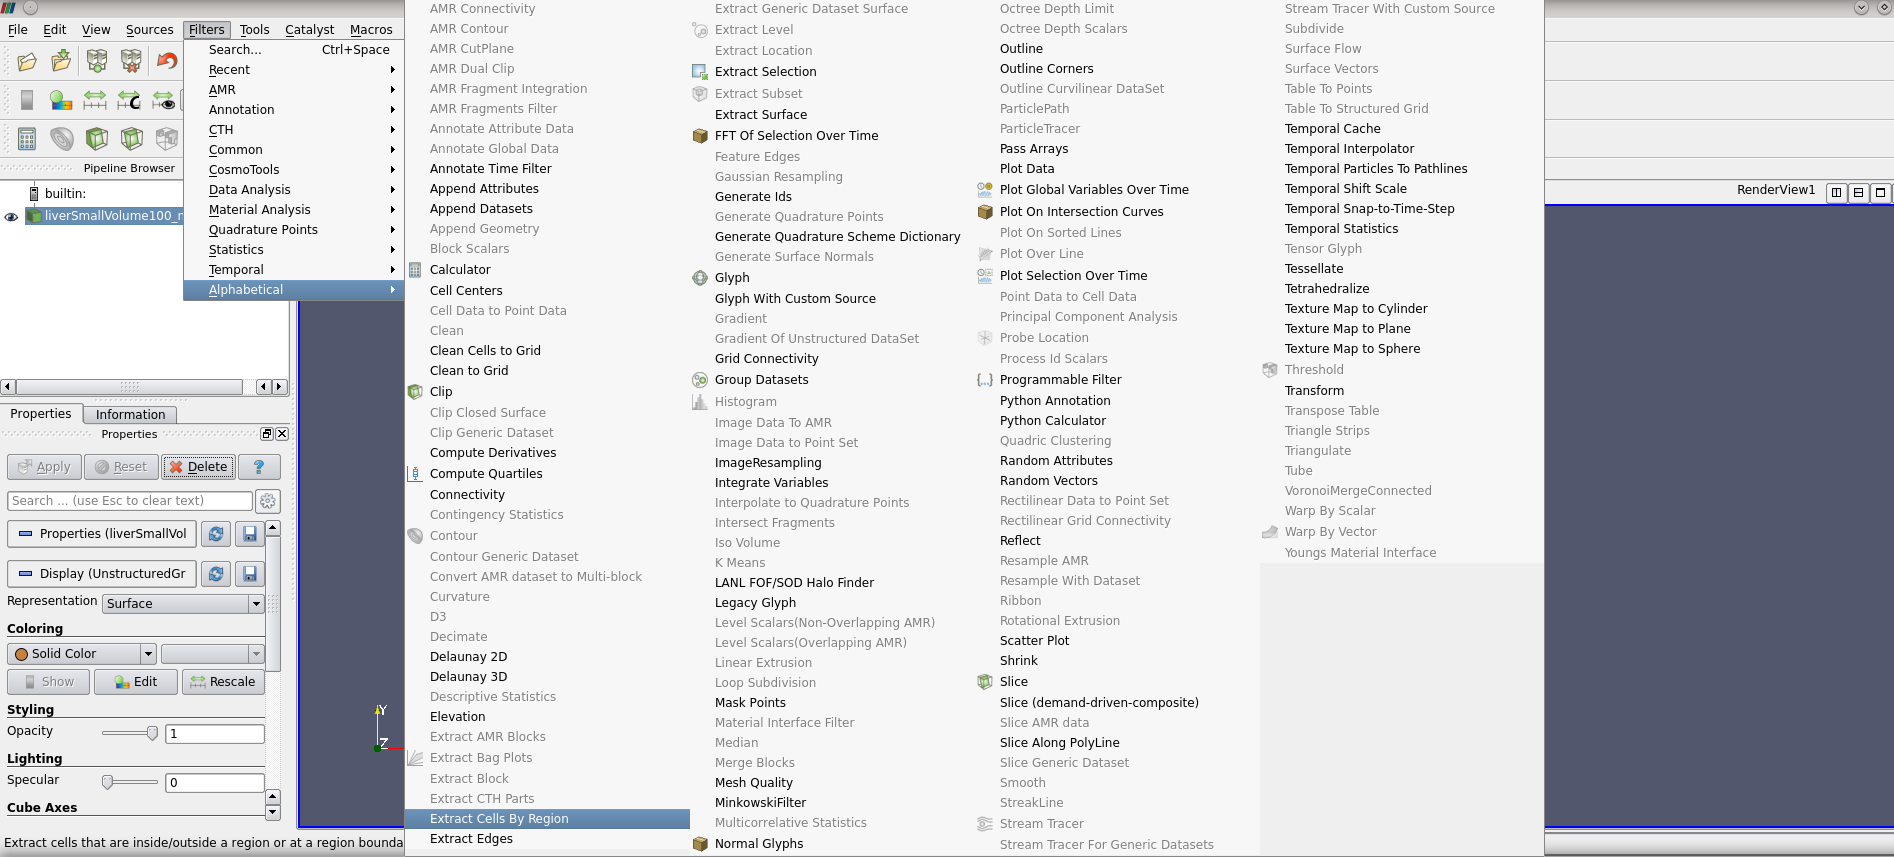
\includegraphics[width=\textwidth]{pictures/paraview_filter.png}
    \caption{Get filter preferences in ParaView.}
    \label{ParaviewFilterScreenshot}
\end{figure}

\newpage

\section{Meshing with quadratic tetrahedral elements}
The MSML contains a powerful and stable workflow in order to convert linear tetrahedral elements to isoparametric quadratic elements (tet10). An example script can be found in "/examples/MeshExample/Tet10/tet10\_runner.py".

Before starting the example from the command line please first make sure that the MSML source is in your Python path:
\begin{lstlisting}[language=sh, breaklines=true]
$ export PYTHONPATH="$PYTHONPATH:/opt/msml/src"
\end{lstlisting}

Then change to the folder that contains the script
\begin{lstlisting}[language=sh, breaklines=true]
$ cd /opt/msml/examples/MeshExample/Tet10
\end{lstlisting}

and run it:
\begin{lstlisting}[language=sh, breaklines=true]
$ python tet10_runner.py
\end{lstlisting}

ParaView can be used again to view the single results and inspect them:
\begin{lstlisting}[language=sh, breaklines=true]
$ cd /opt/paraview/bin/paraview &
\end{lstlisting}